%&main - vim:foldmethod=marker commentstring=%%s foldmarker=<@<,>@>

\def\ifundefined#1{\expandafter\ifx\csname#1\endcsname\relax}
\ifundefined{preambleloaded}% precompiled preamble a la
%
% http://magic.aladdin.cs.cmu.edu/2007/11/02/precompiled-preamble-for-latex/
%
% commands:
%   pdflatex -ini -jobname="main" "&pdflatex preamble.tex\dump"
%   pdflatex -parse-first-line main.tex
%
% - -parse-first-line not needed with TeXlive 2011
% - for latex(1) instead of pdflatex(1), all three occurrences must be
%   replaced
%
%\documentclass[runningheads,orivec]{llncs}
\documentclass{easychair}

\usepackage{xcolor}
\usepackage{amsmath}
\usepackage{amssymb}
\usepackage{mathtools}
\usepackage{float}
\usepackage{tikz}
\usepackage{pgfplots}
\usetikzlibrary{backgrounds,fit,decorations.pathreplacing,snakes,arrows,shapes,automata}
\usetikzlibrary{patterns}
%\usepgfplotslibrary{external}\tikzexternalize
\usepackage{ifthen}
\usepackage{ifpdf}
\usepackage{easpc}
\usepackage{qex}
\usepackage{lskframe}

\ifpdf
\relax
\else
\usepackage{pstricks,pst-node}
\fi





\title{Verification of Fault-Tolerant\\Clock Synchronization Algorithms\\
\normalsize (Benchmark Proposal)}
\author{%
  Sergiy Bogomolov$^{\ddagger}$
  \and
  Christian Herrera$^{\star}$
  \and
  Wilfried Steiner$^{\dagger}$}
\titlerunning{Verification of Fault-Tolerant Clock Synchronization Algorithms}
\authorrunning{Bogomolov, Herrera and Steiner}
\institute{%
  $^{\star}$~Albert-Ludwigs-Universit\"at Freiburg, Freiburg, Germany \\
  $^{\dagger}$~TTTech Computertechnik AG, Chip IP Design, Vienna, Austria \\
  $^{\ddagger}$~IST Austria, Vienna, Austria
} 

% % % % % % % % % % % % % % % % % % % % % % % % % % % % % % % % % % % % % % %

\makeatletter
\newcommand{\todo@box}[1]{\fcolorbox{green!50!black}{green!50!white}{#1}}
\newcommand{\todo}[1]{%
  \begin{center}
  \normalfont%
  \todo@box{\parbox{0.9\textwidth}{\color{black}{\bf TODO}: #1}}
  \end{center}}
\makeatother


% % prelim.tex  % % % % % % % % % % % % % % % % % % % % % % % % % % % % % % %

\newcommand{\ofsane}[1]{\ifthenelse{\equal{#1}{(}}{\errmessage{Hups, '(' as of-macro parameter?}}{}}

\newcommand{\clks}{\mathcal{X}}
\newcommand{\someclks}{X}
\newcommand{\somevars}{V}
\newcommand{\someclksY}{Y}
\newcommand{\clk}{x}
\newcommand{\otherclk}{y}
\newcommand{\thirdclk}{z}
\newcommand{\QE}{\mathcal{QE}}
%
\newcommand{\vars}{\mathcal{V}}
\newcommand{\var}{v}
%
\newcommand{\intexpr}{\psi_\mathit{int}}
%
\newcommand{\Xconstrs}[2][]{\Phi_{#1}(#2)}
\newcommand{\constr}[1][]{\varphi\ifthenelse{\equal{#1}{}}{}{_#1}}
\newcommand{\cconstrs}{\Xconstrs{\clks}}
\newcommand{\cconstr}{\constr_\mathit{clk}}
\newcommand{\vconstrs}{\Xconstrs{\vars}}
\newcommand{\vconstr}{\constr_\mathit{int}}
\newcommand{\constrs}[1][]{\Xconstrs[#1]{\clks,\vars}}
%
\newcommand{\val}{\nu}
\newcommand{\Time}{\mathit{Time}}
%
\newcommand{\clocksofX}[1]{\ofsane{#1}\mathit{clocks}(#1)}
\newcommand{\clocksofta}[1][\ta]{\ofsane{#1}\clks(#1)}
\newcommand{\clocksofrvec}[1][\rvec]{\clocksofX{#1}}
\newcommand{\clocksofconstr}[1][]{\clocksofX{\constr[#1]}}
\newcommand{\varsofX}[1]{\ofsane{#1}\mathit{vars}(#1)}
\newcommand{\varsofrvec}[1][\rvec]{\varsofX{#1}}
\newcommand{\varsofconstr}[1][]{\varsofX{\constr[#1]}}


\newcommand{\locs}{L}
\newcommand{\locsv}{L^{\triangledown}}
\newcommand{\vnstY}[1]{\mathit{vnst}_#1}
\newcommand{\loc}{\ell}
\newcommand{\locv}{\ell_{\triangledown}}
\newcommand{\locva}[1]{\ell_{\triangledown,#1}}
\newcommand{\iloc}[2][]{\loc_{\mathit{ini{#2}\ifthenelse{\equal{#1}{}}{}{#1}}}}
\newcommand{\nstloc}[2][]{\loc_{\mathit{nst{#2}\ifthenelse{\equal{#1}{}}{}{#1}}}}
\newcommand{\tokY}[1][]{\mathit{t}_#1}
\newcommand{\acts}{B}
\newcommand{\comls}{C}
\newcommand{\act}{\alpha}
\newcommand{\locinv}{I}
\newcommand{\edges}{E}
\newcommand{\edge}{e}
\newcommand{\bcacts}{\mathcal{B}}
%
\newcommand{\ta}{\mathcal{A}}
%
\newcommand{\tatupleA}[1][]{%
  (\locs_{#1},\acts_{#1},\clks_{#1},\vars_{#1},}
\newcommand{\tatupleB}[1][]{%
  \locinv_{#1},\edges_{#1},\iloc{})}
\newcommand{\tatuple}[1][]{%
  \tatupleA[#1]\tatupleB[#1]}
%
\newcommand{\rs}{\mathcal{R}(\clks,\vars)}
\newcommand{\rvec}{\vec{r}}
\newcommand{\lvec}{\vec{\loc}}
%
\newcommand{\true}{\mathit{true}}
\newcommand{\false}{\mathit{false}}
%
\newcommand{\edgetuple}[1][]{(\loc_{#1},\act_{#1},\constr_{#1},\rvec_{#1},\loc'_{#1})}
\newcommand{\edgetuplesimpl}{(\loc,\act,\constr,\langle\clk:=0\rangle,\loc')}
\newcommand{\otheredgetuple}[1][]{(\hat{\loc}_{#1},\hat{\act}_{#1},\hat{\constr}_{#1},\hat{\rvec}_{#1},\hat{\loc}'_{#1})}
\newcommand{\otheredgetupleRO}[1][]{(\hat{\loc}_{#1},r_{W}!,\hat{\constr}_{#1},\hat{\rvec}_{#1},\hat{\loc}'_{#1})}
\newcommand{\otheredgetupleRI}[1][]{(\hat{\loc}_{#1},r_{W}?,\hat{\constr}_{#1},\hat{\rvec}_{#1},\hat{\loc}'_{#1})}
\newcommand{\otheredgetupleI}[1][]{(\hat{\loc}_{#1},reset_{W}?,\hat{\constr}_{#1},\hat{\rvec}_{#1},\hat{\loc}'_{#1})}
\newcommand{\otheredgetupleO}[1][]{(\loc_{\resetter{#1}},reset_{#1}!,\hat{\constr}_{#1},\hat{\rvec}_{#1},\nstloc[\resetter{#1}])}
\newcommand{\otheredgetupleR}[1][]{(\ilocR{#1},r_{W}?,\true,\emptyset,\nstlocR{#1})}
%
\newcommand{\locsof}[1]{\ofsane{#1}\locs(#1)}
%\newcommand{\ilocof}[1]{\ofsane{#1}\iloc(#1)}
\newcommand{\edgesof}[1]{\ofsane{#1}\edges(#1)}
\newcommand{\varsof}[1]{\ofsane{#1}\vars(#1)}
\newcommand{\actsof}[1]{\ofsane{#1}\acts(#1)}

\newcommand{\lts}[1]{\ofsane{#1}\mathcal{T}(#1)}
%
\newcommand{\confs}[1]{\ofsane{#1}\mathit{Conf}(#1)}
%\newcommand{\confln}[2]{\langle{#1},{#2}\rangle}
\newcommand{\conf}{c}
\newcommand{\tsconf}{s}
\newcommand{\tsconfdev}{\langle\loc_{\tsconf},\valof{\tsconf}\rangle}
\newcommand{\othertsconf}{r}
\newcommand{\othertsconfdev}{\langle\loc_{\othertsconf},\valof{\othertsconf}\rangle}
%
\newcommand{\iconfs}[1][]{\mathcal{C}_\mathit{ini\ifthenelse{\equal{#1}{}}{}{,#1}}}
%
\newcommand{\labs}{\Lambda}
\newcommand{\lab}{\lambda}
%
\newcommand{\trans}[1]{\xrightarrow{#1}}
\newcommand{\texttrans}[1]{\mathrel{\smash[t]{\trans{#1}}}}
%
\newcommand{\locof}[1]{\ofsane{#1}\loc_{#1}}
\newcommand{\valof}[1]{\ofsane{#1}\val_{#1}}
\newcommand{\confln}[1]{\langle\lvec_{#1}, \valof{#1}\rangle}
%

\newcommand{\comp}{\sigma}
\newcommand{\comps}[1]{\ofsane{#1}\Pi(#1)}
%
\newcommand{\nat}{\mathbb{N}}
\newcommand{\natplus}{\nat^{>0}}
\newcommand{\natnull}{\nat_0}

\newcommand{\parcmp}{\mathrel{\|}}

\newcommand{\nta}{\mathcal{N}}
\newcommand{\mta}{\mathcal{M}}
\newcommand{\sta}{\mathcal{S}}

\newcommand{\res}[1]{\mathcal{RES}_{#1}(\nta)}
\newcommand{\nden}[3][\nta]{\mathcal{DE}^{#2}_{#3}(#1)}
\newcommand{\nde}[3][\ta]{\mathcal{DE}^{#2}_{#3}(#1)}
\newcommand{\lsren}[3][\nta]{\mathcal{LS}^{#2}_{#3}(#1)}
\newcommand{\lcren}[3][\nta]{\mathcal{LC}^{#2}_{#3}(#1)}
\newcommand{\lsre}[2]{\mathcal{LS}^{#1}_{#2}}
\newcommand{\lcre}[2]{\mathcal{LC}^{#1}_{#2}}
\newcommand{\lre}[3][\ta]{\mathcal{LE}^{#2}_{#3}(#1)}
\newcommand{\sre}[1]{\mathcal{SE}_{#1}}
\newcommand{\sren}[3][\nta]{\mathcal{SE}^{#2}_{#3}(#1)}
\newcommand{\cre}[1]{\mathcal{CE}_{#1}}
\newcommand{\cren}[3][\nta]{\mathcal{CE}^{#2}_{#3}(#1)}
\newcommand{\re}[2][]{\mathcal{E}^{#1}_{#2}}
\newcommand{\ren}[3][\nta]{\mathcal{E}^{#2}_{#3}(#1)}
\newcommand{\ul}[1]{\Xi_{#1}}
\newcommand{\congr}[1][\ec]{\equiv_{#1}}
\newcommand{\congrW}[1][W]{\equiv_{#1}}
\newcommand{\hautomaton}{\mathcal{H}}
% % qe.tex  % % % % % % % % % % % % % % % % % % % % % % % % % % % % % % % % %

\newcommand{\qe}{\simeq}

\newcommand{\ecs}[1][\nta]{\mathcal{EC}_{#1}}
%
\newcommand{\ec}{Y}
\newcommand{\ecX}{X}
\newcommand{\otherec}{W}
\newcommand{\rep}{\mathit{rep}}
\newcommand{\seq}[1]{\mathcal{S}_{#1}}
\newcommand{\pt}[1]{\mathcal{P}_{#1}}
\newcommand{\repifynull}{\Gamma_{0}}
\newcommand{\repifyinv}{\Gamma_{\mathit{inv}}}
\newcommand{\repifygrd}{\Gamma}
\newcommand{\repifyct}{\Gamma_{\mathit{c\cdot t}}}

% % wellform.tex  % % % % % % % % % % % % % % % % % % % % % % % % % % % % % %

\newcommand{\Xrloc}[2][]{\mathcal{RL}_{#2}#1}%\ifthenelse{\equal{#2}{\ec}}{(\nta)}{}}
\newcommand{\Nrloc}[2][]{\mathcal{NL}_{#2}#1}%
\newcommand{\rloc}[1]{\Xrloc[^-]{#1}}
\newcommand{\rsuccloc}[1]{\Xrloc[^+]{#1}}

\newcommand{\alg}{\mathcal{K}}
%
\newcommand{\resetter}[1]{\mathcal{R}_{#1}}
\newcommand{\ilocR}[1]{\iloc{\resetter{#1}}}
\newcommand{\locR}[1]{\loc_{\resetter{#1}}}
\newcommand{\nstlocR}[1]{\nstloc{\resetter{#1}}}
\newcommand{\rstX}[2][\ec]{\mathit{rst}_{#1}^{#2}}
\newcommand{\rstI}[1][\ec]{\rstX[#1]{I}}
\newcommand{\rstO}[1][\ec]{\rstX[#1]{O}}
%
\newcommand{\rstIOupd}[1][\edge]{\rho_{#1}}
%
\newcommand{\reset}[1][\ec]{\mathit{reset}_{#1}}
\newcommand{\return}[1][\ec]{\mathit{return}_{#1}}
\newcommand{\rY}[1][\ec]{\mathit{r}_{#1}}
\newcommand{\uY}[1][\ec]{\mathit{u}_{#1}}

% % bisim.tex % % % % % % % % % % % % % % % % % % % % % % % % % % % % % % % %

\newcommand{\sconf}[1]{\mathcal{SC}_{\nta}^{#1}}%\ifthenelse{\equal{#1}{\ec}}{(\nta)}{}}
\newcommand{\dedges}[1]{\mathcal{DE}_{#1}}%\ifthenelse{\equal{#1}{\ec}}{(\nta)}{}}
\newcommand{\othersconf}[1]{\mathcal{SC}_{\nta'}^{#1}}
\newcommand{\Xrseq}[1]{\mathcal{RS}_{#1}}
\newcommand{\rseq}[1]{\Xrseq{#1}}
\newcommand{\rseqpure}[1]{\Xrseq{#1}^\mathit{pure}}
\newcommand{\rseqfullpure}[1]{\Xrseq{#1}^\mathit{full}}
\newcommand{\rseqimpure}[1]{\Xrseq{#1}^\mathit{impure}}

\newcommand{\bigtrans}[1]{\xRightarrow{#1}}
\newcommand{\bigtexttrans}[1]{\mathrel{\smash[t]{\xRightarrow{#1}}}}
%
\newcommand{\Xbsreach}{$\Rightarrow$-reach}
\newcommand{\bsreach}{\Xbsreach{}able}
\newcommand{\bsreaches}{\Xbsreach{}es}

%\newcommand{\BF}{\mathit{BF}}
\newcommand{\BF}{\beta}
\newcommand{\BFof}{\beta}
\newcommand{\CF}{\mathit{CF}}
\newcommand{\EPF}{\mathit{EPF}}
\newcommand{\epfq}[1]{\mathop{\existsOooginool\Diamond} #1}


\newcommand{\wbisimrel}{\mathcal{S}}
\newcommand{\sbisimrel}{\mathcal{S}_{\mathit{str}}}
%\newcommand{\wbisim}{\simeq_\mathit{w}}

\newcommand{\revqe}{\mathit{reverseQE}}
\newcommand{\funqe}{\mathit{QE}}
\newcommand{\devqe}{\mathit{devirQE}}
%
\newcommand{\cons}[1]{\mathit{CONS}_{#1}}
\newcommand{\stable}{\mathit{stable}}
\newcommand{\predelaytrafo}{Z}

% % qeproperties.tex  % % % % % % % % % % % % % % % % % % % % % % % % % % % % % % % % %
\newcommand{\Omg}{\Omega}
\newcommand{\XC}{\mathcal{XC}}
\newcommand{\QC}{\mathcal{QC}}
\newcommand{\CC}{\mathcal{CC}}
\newcommand{\Shi}{\Xi}
\newcommand{\Del}{\Delta}

% % diamond.tex  % % % % % % % % % % % % % % % % % % % % % % % % % % % % % % % % %
\newcommand{\Z}{\mathcal{Z}}
\newcommand{\grph}{G=(V,E)}

% % % % % % % % % % % % % % % % % % % % % % % % % % % % % % % % % % % % % % %

\newcommand{\repval}[4][\val]{#1#3_{#4,\mathit{rep}_{#2}}}
\newcommand{\ECval}[4][\val]{#1#3_{#4,\mathit{QE}_{#2}}}
\newcommand{\nonECval}[4][\val]{#1#3_{#4,\mathit{c}_{#2}}}
\newcommand{\tksval}[2][\val]{#1_{#2,\mathit{tks}}}

\def\preambleloaded{Precompiled preamble loaded.}
\else\typeout{\preambleloaded}\fi

\newenvironment{surgery}{
  \bigskip\hrule\medskip\hrule\smallskip\hrule\bigskip
}{
  \bigskip\hrule\smallskip\hrule\medskip\hrule\bigskip
}

%%\renewcommand{\todo}[1]{}

\begin{document}

\maketitle

\begin{abstract}
In this paper, we propose a benchmark for verification of properties of fault-tolerant clock
synchronization algorithms, namely, a benchmark of a TTEthernet network, 
where properties of the clock synchronization algorithm as implemented in a 
TTEthernet network can be verified, and 
optimization techniques for verification purposes can be applied. Our benchmark, 
which assumes non-faulty components, aims to be a basis for
verifying configurations which include faulty components, information consistency
mechanisms, and for verifying other clock synchronization algorithms.

\end{abstract}

 
\section{Introduction}
\label{sec:intro}
\footnotetext[1]{CONACYT (Mexico) and DAAD (Germany) sponsor the work of this author.}

Distributed real-time systems are present in many commercial hardware and software 
products, e.g. the avionics of the \emph{Orion Space Program}~\cite{Howard}. 
These systems require a generic architecture that complies with
even the most demanding safety-critical real-time requirements.\\ 
\emph{TTEthernet} is an implementation of the traditional \emph{Ethernet} standard
which complies with time-critical, deterministic and safety-critical real-time requirements~\cite{Kopetz}. 
Safety critical systems using the TTEthernet standard rely on the availability 
of a global time base for tolerating faulty behavior of these systems.  
This global time base is a common perception of time for the distributed components of these systems,  
i.e. any two logical clocks of two distributed components must read the same values at any time.
In the TTEthernet standard this common perception of time can be established by 
the periodic synchronization of the physical local clock of each component. 
This synchronization is performed by an internal clock synchronization algorithm~\cite{Kopetz} 
which compensates for the physical
imperfections of these clocks. The maximal difference between the values of 
two logical clocks of two components is the \emph{precision} achieved by the algorithm.

A typical TTEthernet \emph{network} consists of switches and end systems connected by a communication channel,
i.e. a bidirectional point-to-point link. A \emph{standard configuration} consists of end systems 
connected to a single switch, while a \emph{fault-tolerant configuration} consists of end systems 
connected to two independent switches~\cite{Kopetz}. 
Each switch belongs to one and only one communication channel. 
%
In this paper, we present a benchmark inspired by the fault-tolerant configuration 
of a TTEthernet network described in~\cite{Steiner2}, and we use the framework of
hybrid automata~\cite{Alur2,bogomolov-etal:spin2013,bogomolov-etal:cav2012-intro} to analyze and model the exhibiting complex continuous behavior
of a network using this configuration. Our benchmark aims to be a simplified model
where properties of the TTEthernet network, e.g. the precision of the synchronization algorithm, can be verified, and
optimization techniques for verification purposes, e.g. detection and 
reduction of \emph{quasi-dependent variables}~\cite{Herrera3}, can be applied. 

The paper is organized as follows. Section 2 presents an overview of the
clock synchronization algorithm. Section 3 describes our proposed benchmark. 
Section 4 presents the results of our experiments. We conclude in Section 5.
  
\section{Clock Synchronization Overview}
\label{sec:clocksyncoverview}

In a network with a fault-tolerant configuration, switches and end systems assume 
the roles of \emph{Compression Master} (CM), and \emph{Synchronization Master} (SM), 
respectively. Furthermore, each SM is connected to each CM by one and only one communication channel.
In the clock synchronization algorithm which we use, SMs and CMs send information to each other, 
e.g. the current value of the local clock of a given SM, by using \emph{Protocol Control Frames} (PCF).

The clock synchronization algorithm which we use in our benchmark consists of two steps. Firstly, 
each SM sends a PCF to each linked CM. Then each CM extracts from the arrival point in time
of the sent PCF the current value of the local clock of a given SM, 
with this information then the CM executes a first compression function to obtain the median 
from the received clock values of each SM. Secondly, each CM sends in a new PCF the result of 
the first compression function to all SMs, then each SM executes a second compression function
in order to obtain the median of the values received from the CMs. The result of this 
second function is used to correct the value of the clock of each SM. \\
%
The algorithm from above describes the steps for synchronizing clocks in a  
network with non-faulty components, however, the interested reader can find 
in~\cite{Steiner2} a more detailed description of the clock synchronization 
algorithm in networks with faulty components.  

In the next section, we present our benchmark as a network of hybrid automata, 
discuss optimizations for verification purposes, and briefly mention
some possible extensions. 

\section{A Benchmark of a Fault-Tolerant TTEthernet Network}

\label{sec:benchmark}
\begin{figure}[t]%<@<
\centering
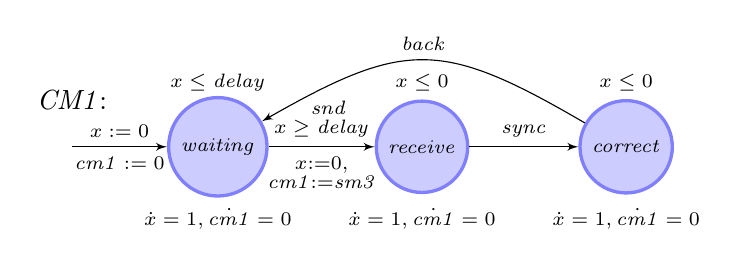
\begin{tikzpicture}[>=latex',join=bevel, scale=0.7]
 \tikzstyle{every state}=     [draw=blue!50,very thick,fill=blue!20]
 \coordinate (init) at (-110bp,77bp);
 \node (A) at (-35bp,77bp) [state] {\scriptsize$\mathit{waiting}$};
 \node (B) at (70bp,77bp) [state] {\scriptsize$\mathit{receive}$};
 \node (C) at (175bp,77bp) [state] {\scriptsize$\mathit{correct}$};
  \node (D) at (22bp,97bp) [] {\scriptsize$\mathit{snd}$};

 \node (Asubscript) at (-35bp, 40bp)  {\scriptsize $\dot{x} = 1, \dot{\mathit{cm1}} = 0$};
 \node (Asuperscript) at (-35bp, 110bp)  {\scriptsize $x \le \mathit{delay}$}; %vertical diff is 24bp
 \node (Bsubscript) at (70bp, 40bp) {\scriptsize $\dot{x} = 1, \dot{\mathit{cm1}} = 0$}; %horizontal diff is 105bp
 \node (Bsuperscript) at (70bp, 110bp)  {\scriptsize $x \le 0$}; 
 \node (Csubscript) at (175bp, 40bp) {\scriptsize $\dot{x} = 1, \dot{\mathit{cm1}} = 0$}; 
 \node (Csuperscript) at (175bp, 110bp)  {\scriptsize $x \le 0$};

 \node (automatonname) at (-110bp, 101bp)  {$\mathit{CM1}$:};


 \draw [->] (init) to node[above] {\scriptsize $x := 0$} node[below] {\scriptsize $\mathit{cm1} := 0$}(A);
 \draw [->] (A) to node[above] {\scriptsize $x \geq \mathit{delay}$} node[below]
 		{ $\substack{x:=0,\\ \mathit{cm1}:= \mathit{sm3}}$}(B);
 \draw [->] (B) to node[above] {\scriptsize$\mathit{sync}$} (C);
 \draw [->] (C) to[distance=3cm, bend right]  node[above] {\scriptsize$\mathit{back}$} (A);

\end{tikzpicture}

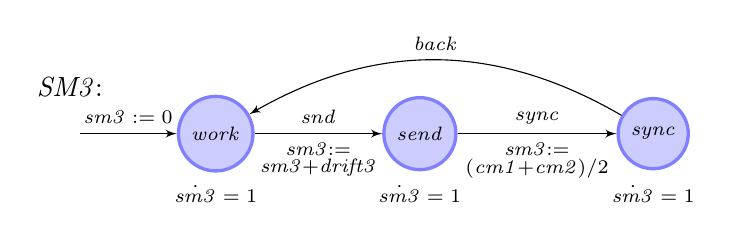
\begin{tikzpicture}[>=latex',join=bevel,scale=0.7]
 \tikzstyle{every state}=     [draw=blue!50,very thick,fill=blue!20]
 \coordinate (init) at (-105bp,77bp);
 \node (A) at (-35bp,77bp) [state] {\scriptsize$\mathit{work}$};
 \node (B) at (70bp,77bp) [state] {\scriptsize$\mathit{send}$};
 \node (C) at (190bp,77bp) [state] {\scriptsize$\mathit{sync}$};

 \node (Asubscript) at (-35bp, 46bp)  {\scriptsize $\dot{\mathit{sm3}} = 1$};
 \node (Bsubscript) at (70bp, 46bp) {\scriptsize $\dot{\mathit{sm3}} = 1$}; %horizontal diff is 105bp
 \node (Csubscript) at (190bp, 46bp) {\scriptsize $\dot{\mathit{sm3}} = 1$}; 

 \node (automatonname) at (-110bp, 101bp)  {$\mathit{SM3}$:};


 \draw [->] (init) to node[above] {\scriptsize $\mathit{sm3}:=0$} (A);
 \draw [->] (A) to node[above] {\scriptsize $\mathit{snd}$} 
 				node[below]{$\substack{\mathit{sm3}:=\\ \mathit{sm3}+\mathit{drift3}}$}(B);
 \draw [->] (B) to node[above] {\scriptsize $\mathit{sync}$} 
 					node[below]{$\substack{\mathit{sm3}:= \\ (\mathit{cm1}+\mathit{cm2})/2}$}(C);
 	 \draw [->] (C) to[bend right]  node[above] {\scriptsize$\mathit{back}$} (A);				
\end{tikzpicture}

\vspace*{-1em}
\caption{Components $\mathit{CM1}$ and $\mathit{SM3}$ of a network with two CMs and five SMs.}
\label{fig1}
\end{figure}%>@>

In the following, we use the definitions of hybrid automata as described in~\cite{Herrera3}.
For simplicity we propose a typical industrial network of hybrid automata using a fault-tolerant configuration
with two CMs, namely, $\mathit{CM1}$ and $\mathit{CM2}$, 
and five SMs from $\mathit{SM1}$ to $\mathit{SM5}$. 
In Figure~\ref{fig1} automaton $\mathit{CM1}$ consists of the 
real variables $x$ (the local clock with \emph{rate} 1), and $\mathit{cm1}$ which stores the result of the first compression function, and 
the locations $\mathit{waiting}$ (initial), $\mathit{receive}$ and $\mathit{correct}$, while 
automaton $\mathit{SM3}$ consists of the real variables $\mathit{sm3}$ (the local clock with rate 1);  \emph{drift3}  which ranges from 
$-\mathit{maxdrift}$ to $\mathit{maxdrift}$, where $\mathit{maxdrift}$ describes the absolute value of the maximum 
drift offset that a SM's clock can achieve before the execution of the synchronization algorithm, 
and the locations $\mathit{work}$ (initial), $\mathit{send}$ 
and $\mathit{sync}$. The exchange of PCFs between CMs and SMs is realized in our benchmark
by using edges in SMs and CMs labeled with $\mathit{snd}$ and $\mathit{sync}$. 
The rest of the CMs and SMs follow a similar structure.

At the start of the system each automaton delays exactly $\mathit{delay}$ time units, 
with $\mathit{delay}>0$, at the unique location where a delay greater than 0 time units is possible, namely, at 
its initial location. Then after this delay 
the CMs and SMs respectively transit simultaneously to locations $\mathit{receive}$ and 
$\mathit{send}$ by taking the edges labeled with $\mathit{snd}$.
By performing this transition each SM sends the drifted value of their clocks to both CMs. 
Then $\mathit{CM1}$ and $\mathit{CM2}$ store in their variables $\mathit{cm1}$
and $\mathit{cm2}$, respectively, the result of the first compression function, which in Figure~\ref{fig1}
we assume is the drifted value of the clock $\mathit{sm3}$. 
The second compression function, performed to correct the value of the clock of each SM, 
is executed when CMs and SMs transit simultaneously to locations
$\mathit{correct}$ and $\mathit{sync}$, respectively, by taking the edges labeled with $\mathit{sync}$.
Finally, all automata return to their initial location by simultaneously taking the 
edges labeled with $\mathit{back}$.

It is important to point out that we assume non-faulty components, hence, 
consistency mechanisms for detecting PCFs from faulty components are not included in our benchmark.

\subsection{Optimization for Verification Purposes}

Our benchmark is a candidate for the optimization techniques that we have presented in~\cite{Herrera3}, namely,
detection and reduction of quasi-dependent variables. Quasi-dependency of variables is a generalization 
of \emph{quasi-equality} of clocks~\cite{Herrera,Herrera2,Herrera4}. Intuitively, between two variables $\clk$ and $\otherclk$ 
of a hybrid automaton $\hautomaton$, there exists a quasi-dependency, namely, $\clk$ quasi-depends
on $\otherclk$ via function $f$, if and only if at all runs of $\hautomaton$ and at all points in time,
the value of $\clk$ is the value of $f$ applied to the value of $\otherclk$, except when the value of 
$\otherclk$ is determined by an update action. 

The technique in~\cite{Herrera3} allows us to detect in our TTEthernet 
network two sets of quasi-dependent variables, namely,
the set consisting of clocks from each SM, and the set consisting of clocks from each CM. 
This detection allows us as well to implement a reduction of 
the detected quasi-dependent variables together with a syntactical transformation of 
the original network, in order to produce a transformed network where the original complexity is reduced,
and where properties of the original network are reflected, that is, a forbidden configuration is reachable in
the transformed network if and only if it is reachable in the original network. The most remarkable result of this 
transformation is a dramatic performance improvement of the verification time of properties of the transformed network. 
We refer the interested reader to~\cite{Herrera3} for more details on the detection and reduction of quasi-dependent
variables. 

\subsection{Possible Extensions of the Benchmark}

In the following, we mention some possible extensions and uses for our benchmark:
\begin{enumerate} 
\item it can be used as a basis for modeling TTEthernet networks where we can verify the
precision of the synchronization algorithm under failures of a single SM, a single CM, and
under concurrent SM and CM failures as studied in~\cite{Steiner2},   
\item it can be also used as a basis for verifying 
clock synchronization algorithms like the \emph{interactive convergence algorithm}\cite{lamport}
and the \emph{byzantine clock synchronization}\cite{lamport},
\item it can be useful for studying
and implementing the elimination of the remaining syntactical assumptions for
networks of hybrid automata, similar to the work for networks of timed automata~\cite{Alur} 
with quasi-equal clocks as described in~\cite{Herrera4}, and
\item  it can be used for scalability analysis 
by introducing additional CMs and SMs.
\end{enumerate} 

\subsection{Open Problems of the Benchmark}
Note that in our benchmark we assume that the rate of each clock is 1. However, in practice this assumption
may not always hold due to the imperfection of the physical clocks, for instance, the clock of a SM may have 
rate 1 for at most $n$ time units before dropping below 1, that is, that clock will tick slower than rate 1 after $n$ time units.
In this case a rate correction algorithm as in~\cite{Steiner3} will correct the rate of that clock. 
A more realistic benchmark would consider scenarios where the clock of a given SM has several rates before the execution
of the synchronization algorithm. However, remains unclear how to detect and reduce quasi-dependent variables in benchmarks with
the mentioned scenarios, since that detection and reduction assumes that the rate of the variables in a model is constant at all points in time. Therefore, further studies wrt.\ quasi-dependent variables with different rates for the same variables are required.      
 
\section{Experiments}
In the following section, we present the results of our experiments, where our aim is to show that
in our benchmark we have: (a) verified that the precision of the synchronization algorithm holds and, 
(b) applied the techniques for detecting and reducing quasi-dependent variables. 
We have verified the precision of the synchronization algorithm in settings of our benchmark with 2 CMs and from 5 to 30 SMs. 
We recall that our benchmark is a fault-tolerant TTEthernet network with non-faulty components. 
In this benchmark, we verify that the maximal difference between the values of any two logical clocks of two SMs is bounded by 
$2*\mathit{maxdrift}$, as reported in~\cite{Steiner2}, 
i.e.\ $\forall i\neq j\in\nat\bullet \ sm_i > sm_j \implies sm_i-sm_j \leq 2*\mathit{maxdrift} $.
%
In addition, in order to enable efficient handling of large scale
benchmark instances, we have applied a model transformation based on
quasi-dependent variables~\cite{Herrera3}. 
%
%% Additionally, we have transformed each setting, where we have detected and reduced the number of 
%% quasi-dependent variables. 
The results for both, original and transformed networks, are reported in 
Table~\ref{Table1}. In this table, we compare the analysis runtime needed by the model checker 
SpaceEx~\cite{Frehse,bogomolov-et-al-sttt2015,DBLP:conf/hvc/BogomolovFGGPPS14}
%%  in 2,000 iterations
 for the original and the transformed networks (the latter denoted in the table by the suffix K). 
Note that transformed models use only one clock for the CMs and one clock for the SMs.
%
We observe that the transformation leads to a drastic performance improvement due to the reduction of quasi-dependent variables.   

%% We refer the interested reader to~\cite{Herrera3} for a detailed explanation regarding the reduction of the 
%% verification runtime in models transformed by the quasi-dependent variables approach.
  
\begin{table}[H]
\centering
\setlength{\tabcolsep}{4pt}
%\raisebox{3ex}{%
\begin{tabular}[b]{ l r r r  | l r r r r r r }
\hline\hline
\multicolumn{1}{l}{ Network} & \multicolumn{1}{c}{{C}} & \multicolumn{1}{c}{M} &\multicolumn{1}{c|}{ $t(s)$}  \\[0.5ex]
\cline{1-4}
 \textit{TT-5}   & \makebox[0pt][r]{7}& 3.0& 31.32	&\textit{}   & &  &  	\\
 \textit{TT-5K}   & \makebox[0pt][r]{2}&  2.9&  11.96&\textit{}   & &  &  	\\
 \textit{TT-20}   & \makebox[0pt][r]{22}&  3.0&  124.08	
  &\multicolumn{4}{l}{\quad\footnotesize
    Experimental environment: Intel~i3,}  	\\
 \textit{TT-20K}   & \makebox[0pt][r]{2}& 3.0& 12.11 
  &\multicolumn{4}{l}{\quad\footnotesize
    2.3\,GHz, 3\,GB, Ubuntu~11.04,}  	\\
 \textit{TT-30}   & \makebox[0pt][r]{32}& 3.1& 201.21
  &\multicolumn{4}{l}{\quad\footnotesize
    SpaceEx server VM (VMX) v0.9.8b / PHAVer scenario.}  	\\
 \textit{TT-30K}   & \makebox[0pt][r]{2}& 3.0& 12.57  \\
\cline{1-4}
\end{tabular}

\caption{
  Row X-$N(K)$ gives the figures for case study X with $N$ components, the suffix `K' denotes the models after the quasi-dependent variables transformation, 
  %
  `C' gives the number of clocks in the model, 
  `M' memory usage in MB for the analysis,
  and `$t(s)$' verification time in seconds.
  %
  Detection of clocks does not contribute to the verification time.
}
\label{Table1}
\end{table}
\section{Conclusion}

We have presented a benchmark inspired by the fault-tolerant configuration 
of a TTEthernet network, and we have used the framework of
hybrid automata to analyze and model the exhibiting complex continuous behavior
of that network. Our benchmark is a simplified model
where properties of the TTEthernet network can be verified, and
optimization techniques for verification purposes can be applied.  
The  benchmark can incorporate new CMs and SMs and be used in scalability analysis. 
Furthermore, our benchmark can be extended and used for verifying 
synchronization algorithms under failures of its components. Interesting open problems
wrt.\ this benchmark require further studies, e.g.\ clocks in components with multiples rates 
for some time units and their implications wrt.\ detection and reduction of quasi-dependent variables. 








%% \clearpage

\bibliographystyle{unsrt}
\vspace*{-5px}
\bibliography{main}
\clearpage
\end{document}



